\subsubsection{\stid{4.14} VeloC: Very Low Overhead Checkpointing System}

\paragraph{Overview.}
The VeloC-SZ project aims to provide VeloC, a high-performance,
scalable checkpoint/restart framework that leverages multi-level
checkpointing (the combination of several resilience strategies and
heterogeneous storage) to ensure that ECP applications run to
completion with minimal performance overhead. It delivers a
production-ready solution that increases development productivity by
reducing the complexity of having to deal with a heterogeneous storage
stack and multiple vendor APIs. VeloC offers a client library that can
be used by the applications to capture local application states, which
are then coordinated and persisted using a resilience engine.  VeloC
runs the resilience engine asynchronously, which overlaps a large part
of the checkpointing with the application runtime, thereby reducing
its overhead. An overview of the architecture of VeloC is depicted
in Figure~\ref{fig:veloc:arch}.

VeloC has been released and shows significant lower checkpointing
overhead for several ECP applications, such as HACC, LatticeQCD,
EXAALT. 

\paragraph{Key Challenges.}
VeloC faces several key challenges:
\vspace{-1em}

\paragraph{\emph{I/O bottlenecks:}} applications typically employ
simple checkpoint-restart mechanisms to survive failures that directly
use a parallel file system. With diminishing I/O bandwidth available
per core, this leads to high checkpointing overhead and is not
sustainable.
\vspace{-1em}

\paragraph{\emph{Deep heterogeneous storage:}} To compensate for
diminishing parallel file system I/O bandwidth per core, the storage
stack is becoming increasingly deeper and heterogeneous: node-local
NVRAM, burst buffers, key-value stores, etc. However, the variety of
vendors and performance characteristics make it difficult for
application developers to take advantage of it.
\vspace{-1em}

\paragraph{\emph{Restart-in-place:}} a majority of failures affect
only a small part of the nodes where the job is running. Therefore,
reusing the surviving nodes to restart from the latest checkpoint
immediately after a failure is more efficient than submitting a new job,
which may wait in the batch queue.
\vspace{-1em}

\paragraph{\emph{Portability and robustness:}} applications need to
run on a variety of supercomputing architectures, each featuring
distinct capabilities. Their critical data structures that need to be
checkpointed are constantly growing in size and complexity. Therefore,
a flexible checkpointing solution is needed that can adapt to a
variety of scenarios and configurations without sacrificing
performance and scalability.

\paragraph{Solution Strategy}

To address these challenges, VeloC adopts the following principles:
\vspace{-1em}

\paragraph{\emph{Multi-level checkpointing:}} is based on the idea
that a majority of failures can be mitigated without involving the
parallel file system: node-local checkpoints can be used to recover
from software bugs, replication/erasure coding can be used to recover
from most combinations of node failures. This reduces the frequency of
checkpointing to the parallel file system and therefore the I/O
bottlenecks.
\vspace{-1em}

\paragraph{\emph{Asynchronous mode:}} once a node-local checkpoint has
been written, applications do not need to wait for replication,
erasure coding or writes to the parallel file system: these can be
applied in the background, while the application continues
running. However, in this case, it is important to minimize
interference with the application execution.
\vspace{-1em}

\paragraph{\emph{Transparent use of heterogeneous storage:}} we
developed several techniques that can leverage a variety of local
storage (in-memory file systems, flash storage) and external storage
(burst buffers, key-value stores, parallel file systems)
options. These techniques select the best available storage options,
tune them with the optimal parameters and leverage any vendor-specific
API if needed to transfer data.
\vspace{-1em}

\paragraph{\emph{Job scheduler integration:}} to implement
restart-in-place, we have developed a series of scripts that interact
with a variety of job schedulers to run jobs with spare nodes,
continue execution on failures, restart on the surviving nodes and
spares using the fastest possible recovery strategy (which ideally
avoids reading checkpoints from the parallel file system). This is
transparent to the users.
\vspace{-1em}

\paragraph{\emph{Declarative API and automated serialization:}} we
offer a simple API that enables users to either manually capture
checkpoints into files or to define memory regions that are
automatically serialized into checkpoint files.
\vspace{-1em}

\paragraph{\emph{Modular design:}} applications link with a client
library that is responsible to manage local checkpoints, while a
separate engine is responsible to employ the rest of the resilience

strategies as plugable modules. This simplifies the implementation
of the asynchronous mode, it enables users the flexibility to choose any
combination of resilience strategies, as well as, to customize their
checkpointing pipeline (e.g., add new post-processing operations such
as analytics or compression).

\paragraph{Recent Progress}

We met and closely collaborated with several ECP application teams in
an effort to address their checkpointing needs. Most of our current
efforts involve the HACC, LatticeQCD, and EXAALT teams. Starting from
our previous efforts to isolate the checkpointing code into an optional
plugin within the application (which is notably the case of HACC, where
we integrated VeloC as a CosmoTools plugin), we developed an automated
deployment for the components of VeloC, which has two advantages: (1)
it eliminates the need to change the application deployment scripts
to launch the active backend; (2) it enables the application to decide
the VeloC configuration dynamically at runtime.

\begin{wrapfigure}{l}{0.47\textwidth}
  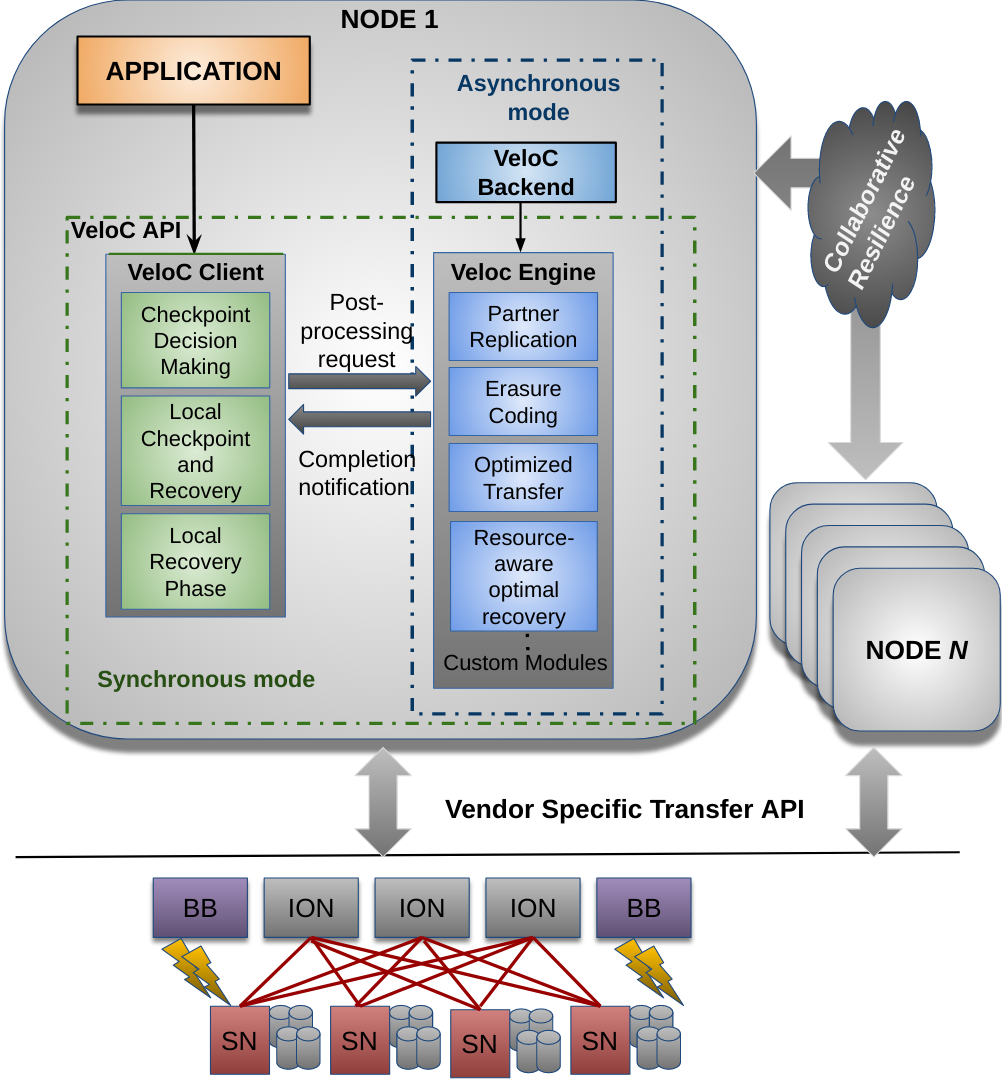
\includegraphics[width=0.4\textwidth]{projects/2.3.4-DataViz/2.3.4.14-VeloC-SZ/veloc-arch}
  \caption{VeloC: Architecture}%
  \label{fig:veloc:arch}%
\end{wrapfigure}

Furthermore, we added several new capabilities. First, we have added
a \emph{checksumming} module that verifies the integrity of the checkpoints
This is done asynchronously to minimize the overheads of using this capability.
Second, we have refactored the control plane that facilitates the communication
between the VeloC clients and the active backends to include two new alternatives:
(1) a lightweight communication protocol based on UNIX sockets for the case
when the active backend is co-deployed with the VeloC clients; an RPC-based
communication protocol based on Mercury/Thallium that enables the active
backend to be deployed on separate nodes. Both alternatives complement the
existing default control plane implemented using POSIX shared memory.

In addition, we have added several new features that facilitate better
integration with the ECP ecosystem. In addition to continuous
integration based on Travis (linked to our public GitHub repository),
we designed and developed a test suite for VeloC that verifies the
correctness in a multi-node setup on the ECP testbeds using the
continuous integration platform provided by ECP (which is configured to
mirror the GitHub repository). We are also providing a Spack
installation package that is part of the OpenHPC distribution.

We also started several exploratory directions that resulted in
several research publications. Notably, we explored how to optimize
the checkpoint interval for our multi-level checkpointing strategies
used in VeloC. In this context, we devised a technique to reduce the
simulation cost of various failure scenarios for a wide range of
parameters using machine learning ~\cite{MLCkpt20}. Furthermore, we
also developed specialized checkpointing approaches for deep learning
applications.  In particular, we explored how to take advantage of
specific properties (e.g. multiple model replicas in the case of
data-parallel training) in order to reduce the asynchronous
checkpointing overhead. Our work DeepFreeze~\cite{DeepFreeze20}
illustrates such techniques based on the idea of augmenting the
execution graph with fine-grain tensor copy operations, which then be
asynchronously flushed to stable storage. We plan to integrate such
approaches with ECP CANDLE, which relies primarily on deep learning.

\paragraph{Next Steps}
We are working towards several goals: (1) providing a set of C++
client interfaces as well as automated serialization support for
common C++ data structures (notably from the STL); (2)
investigate and apply mitigation mechanisms for features that
are missing or perform suboptimally (notably multiple concurrent 
MPI instances); (3) continue hardening the integration with
existing ECP applications and automated testing infrastructure.
In parallel, we will continue to collaborate with the ECP application
teams to address new requirements should they arise.